\chapter{TINJAUAN PUSTAKA}
\label{chap:tinjauanpustaka}

% Ubah bagian-bagian berikut dengan isi dari tinjauan pustaka

\section{Penelitian Terdahulu}
\label{sec:penelitianterdahulu}
% \begin{enumerate}
%   \item \emph{Deep Learning Based Safety Helmet Detection in Engineering Management Based on Convolutional Neural Networks}
%   \par Li dan teman teman pada tahun 2020 melakukan penelitian untuk metode deteksi helm keselamatan kerja secara real time berbasis deep learning pada lokasi konstruksi. Li dan teman – teman menggunakan SSD-MobileNet yang berbasis dari CNN. Menggunakan dataset yang berjumlah 3261 gambar helm keselamatan. SSD- Mobilenet dipilih dibanding R-CNN dengan maksud pendeteksian yang lebih cepat dan cocok untuk real – time walau tidak seakurat R-CNN. \cite{li2020deep}
  
%   \item Deteksi Penggunaan Helm Pada Pengendara Bermotor Berbasis Deep Learning
%   \par Yusuf Umar pada tahun 2020 melakukan penelitian tentang deteksi penggunaan helm pada pengendara bermotor. Pada penelitiannya menggunakan YOLOv3 yang berbasis dari CNN. Pada sistem yang dikembangkan dapat memberikan bounding box ke pengendara lalu dalam bounding box pengendara terdapat boundbox lain dari kepala hingga dada pengendara untuk mendeteksi penggunaan helm motor ada atau tidak. \cite{hanafi2020deteksi}

%   \item \emph{Safety Helmet Detection Based on YOLOv5}
%   \par Zhou dan teman - teman pada awal tahun 2021 yang berupa penelitian deteksi helm keselamatan kerja yang berbasis dari YOLOv5. Pada penelitiannya Zhou dan teman - teman melakukan perbandingan dengan 4 model dari YOLOv5 yang meliputi YOLOv5s, YOLOv5m, YOLOv5l, dan YOLOv5. Selain itu Zhou dan teman - teman menggunakan dataset yang berisi 6054 gambar yang dikumpulkan dari
%   internet dan di anotasi sendiri. Label anotasinya ada dua yaitu "Alarm" yang merupakan kepala tanpa helm dan
%   "helmet" yang merupakan kepala dengan helm keselamatan kerja\cite{zhou_zhao_nie_2021}.
% \end{enumerate}

\subsection{\emph{Deep Learning Based Safety Helmet Detection in Engineering Management Based on Convolutional Neural Networks}}
\label{subsec:deeplearningli2020}

Li dan teman teman pada tahun 2020 melakukan penelitian untuk metode deteksi helm keselamatan kerja secara real time berbasis deep learning pada lokasi konstruksi. Li dan teman – teman menggunakan SSD-MobileNet yang berbasis dari CNN. Menggunakan dataset yang berjumlah 3261 gambar helm keselamatan. SSD- Mobilenet dipilih dibanding R-CNN dengan maksud pendeteksian yang lebih cepat dan cocok untuk real – time walau tidak seakurat R-CNN. \cite{li2020deep}

\subsection{Deteksi Penggunaan Helm Pada Pengendara Bermotor Berbasis Deep Learning}
\label{subsec:deteksihelmmotoryusuf}
\par Yusuf Umar pada tahun 2020 melakukan penelitian tentang
 deteksi penggunaan helm pada pengendara bermotor. 
 Pada penelitiannya menggunakan YOLOv3 yang berbasis dari CNN. 
 Pada sistem yang dikembangkan dapat memberikan bounding box ke 
 pengendara lalu dalam bounding box pengendara terdapat boundbox 
 lain dari kepala hingga dada pengendara untuk mendeteksi 
 penggunaan helm motor ada atau tidak. \cite{hanafi2020deteksi}

\subsection{\emph{Safety Helmet Detection Based on YOLOv5}}
\label{subsec:safetyhelmetyolov5}
\par Zhou dan teman - teman pada awal tahun 2021 yang berupa penelitian deteksi helm keselamatan kerja yang 
berbasis dari YOLOv5. Pada penelitiannya Zhou dan teman - teman melakukan perbandingan dengan 4 model dari 
YOLOv5 yang meliputi YOLOv5s, YOLOv5m, YOLOv5l, dan YOLOv5. Selain itu Zhou dan teman - teman menggunakan 
dataset yang berisi 6054 gambar yang dikumpulkan dari internet dan di anotasi sendiri. 
Seperti yang ditunjukan pada Gambar~\ref{fig:zhouimage}, terdapat dua kelas yaitu "Alarm" yang merupakan kepala tanpa helm dan
"helmet"  yang merupakan kepala dengan helm keselamatan kerja\cite{zhou_zhao_nie_2021}.

\begin{figure}[ht]
    \centering
    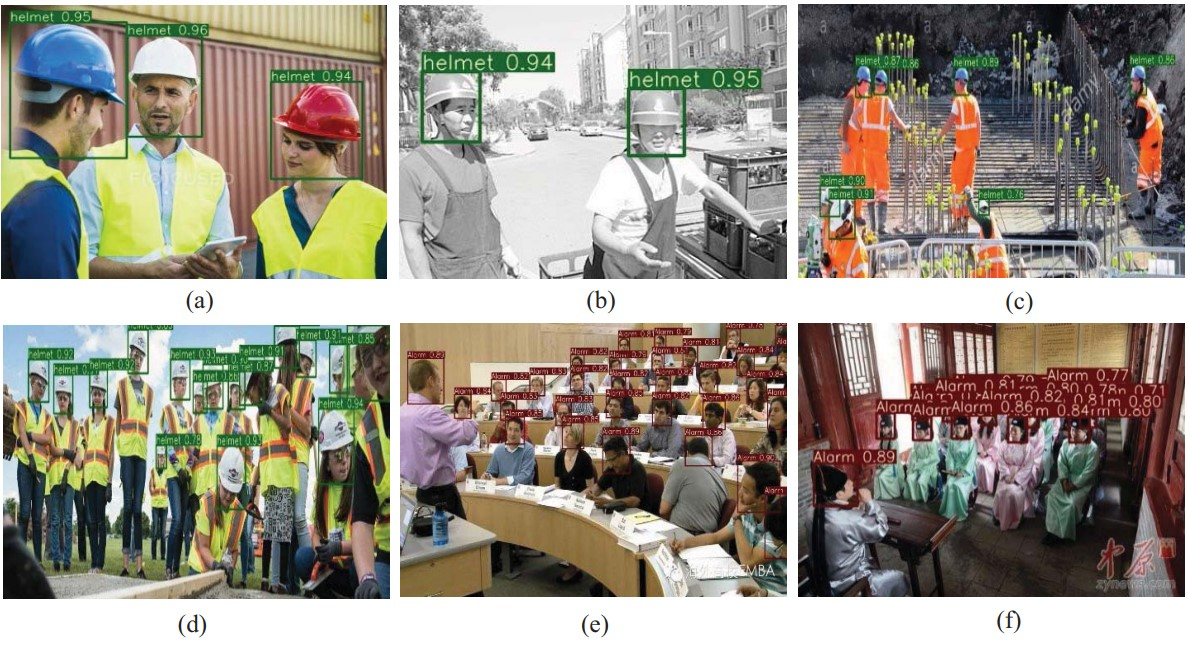
\includegraphics[scale=0.7]{gambar/zhou_le.jpg}
    \caption{Hasil Deteksi Helm Keselamatan Kerja pada penelitian oleh Zhou dan kawan - kawan}
    \label{fig:zhouimage}  
\end{figure}

% % Contoh input gambar
% \begin{figure}[ht]
%   \centering

%   % Ubah dengan nama file gambar dan ukuran yang akan digunakan
%   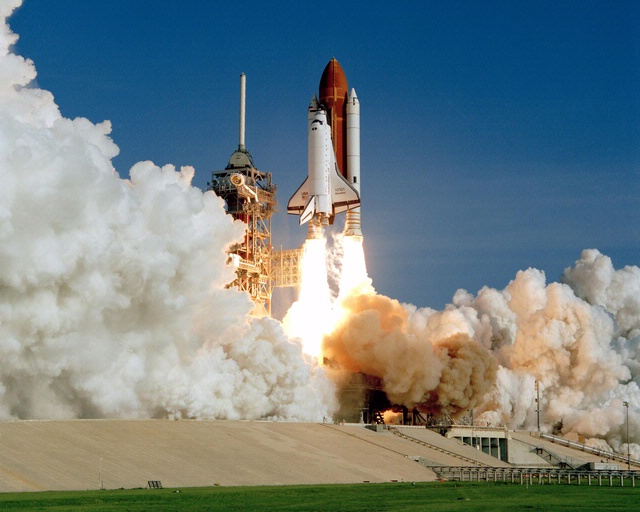
\includegraphics[scale=0.35]{gambar/roketluarangkasa.jpg}

%   % Ubah dengan keterangan gambar yang diinginkan
%   \caption{Peluncuran roket luar angkasa \emph{Discovery} \citep{roketluarangkasa}.}
%   \label{fig:roketluarangkasa}
% \end{figure}

% Roket luar angkasa merupakan \lipsum[1]

% \emph{Discovery}, Gambar \ref{fig:roketluarangkasa}, merupakan \lipsum[2]

% Per Teori Penunjang dibuat section baru

\section{Helm Keselamatan Kerja}
\label{sec:helmkeselamatankerja}

\begin{figure}[ht]
    \centering
    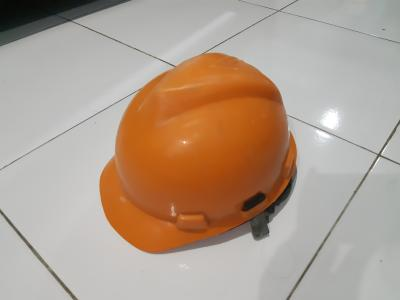
\includegraphics[scale=0.7]{gambar/safety_helmet.jpg}
    \caption{Helm Keselamatan Kerja}
    \label{fig:helmkeselamatankerja}  
\end{figure}

Helm Keselamatan Kerja seperti helm atau pelindung kepala pada umumnya memiliki kemampuan untuk 
melindungi kepala pengguna. Menurut surat dari Menteri Tenaga Kerja dan Trasmihrasi nomor PER. PER. 08/MENVIII/2010, 
jenis – jenis alat perlindungan diri salah satunya yaitu Alat Pelindung Kepala yang dimana contoh bentuk
nya yaitu helm keselamatan kerja atau safety helmet diantara alat pelindung lainnya \cite{suratkementriantenagakerja}. 
Saat digunakan dengan tepat, helm dapat menyerap dampak benturan yang mengurangi gaya yang disalurkan ke kepala hingga 10 persen dari dampak benturan aslinya. \cite{kim2018safety}

Badan Standar Dunia dari Amerika, \emph{Occupational Safety and Health Administration} atau OSHA mengatur 
standardisasi Helm Keselamatan Kerja di pedoman ANSI/ISEA Z89.1-2014. Dalam pedoman memiliki dua tipe 
klasifikasi perlindungan yaitu TIPE I yang merupakan perlindungan dari atas dan TIPE II yang merupakan 
perlindungan lateral atau menyamping yang dimana kedua tipe dites untuk benturan dan ketahanan dari 
penetrasi. Untuk tipe II meliputi kemampuan meredam benturan dari depan , belakang, dan samping. 
Selain itu TIPE II juga meliputi pertahanan penetrasi off-center dan ketahanan tali dagu \cite{american1997american}.

Selain dari 2 tipe perlindungan dari benturan, standardisasi ANSI/ISEA Z89.1-2014 juga meliputi 3 kelas tingkat isolasi listrik yaitu \cite{american1997american}:
\begin{enumerate}
    \item \emph{G Class} yang tahan sampai 2.200 volt
    \item \emph{E Class} yang tahan sampai 20.000 volt
    \item \emph{C Class} yang sama sekali tidak memiliki tingkat isolasi listrik
\end{enumerate}

Dari situ dapat disimpulkan bahwa helm keselamatan kerja memiliki manfaat yang besar dalam melindungi kepala personel konstruksi.

\section{Peraturan Menteri Tenaga Kerja dan Transmigrasi Republik Indonesia tentang Alat Pelindung Diri}
\label{sec:peraturanapd}

\par Peraturan Menteri Tenaga Kerja dan Transmigrasi Republik Indonesia NOMOR PER.08/MEN/VII/2010 mengatur tentang alat pelindung diri.
Peraturan ini meliputi pihak - pihak yang terlibat, kewajiban penyediaan APD, peralatan yang termasuk APD, dan karakteristik tempat
yang diwajibkan APD \cite{suratkementriantenagakerja}. Pada pasal 3 ayat 1, disebutkan alat - alat yang termasuk sebagai alat pelindung diri
yaitu :

\begin{enumerate}[nolistsep]
    \item pelindung kepala
    \item pelindung mata dan muka
    \item pelindung telinga
    \item pelindung pernapasan beserta kelengkapannya
    \item pelindung tangan
    \item pelindung kaki
\end{enumerate}
Dimana pelindung kepala ini meliputi helm keselamatan kerja atau \emph{hardhat}.

\section{Peraturan Menteri Pekerjaan Umum tentang Pedoman Sistem Manajemen Keselamatan dan Kesehatan Kerja (SMK3) Konstruksi Bidang Pekerjaan}
\label{sec:peraturansmk3}

\par Peraturan Menteri Pekerjaan Umum NOMOR : 05/PRT/M/2014 mengatur Pedoman Sistem Manajemen Keselamatan dan Kesehatan Kerja (SMK3) Konstruksi Bidang Pekerjaan.
Peraturan ini meliputi ketentuan umum tentang keselamatan dan kesehatan kerja konstruksi, sistem manajemen K3, pekerjaan konstruksi
,ahli K3 Konstruksi, petugas K3 Konstruksi, potensi bahaya, dan risiko K3. Dijelaskan pada pasal 6 ayat 1 dan 2 bahwa Ahli K3 atau Petugas K3 wajib dilibatkan pada konstruksi
dengan potensi bahaya tinggi atau rendah.


\section{Convolutional Neural Network}
\label{sec:convolutionalneuralnetwork}

\par \emph{Convolutional Neural Network} adalah metode deep learning yang didesain untuk rekognisi pada data dua 
dimensi yang dimana umumnya berupa gambar visual (tetapi tidak harus berupa gambar) dan untuk klasifikasi.
Convolutional Neural Network memiliki kedalaman jaringan yang tinggi sehingga juga bisa termasuk sebagai \emph{Deep Neural Network}.
Jika dibandingan dengan \emph{Multilayer Perceptron} atau MLP, kemampuan CNN untuk klasifikasi citra lebih baik dibandingkan dengan MLP karena MLP tidak memiliki
kemampuan untuk menyimpan \emph{spatial information} dari gambar dimana satu \emph{pixel} pada gambar dianggap sebagai satu fitur
terpisah atau independen \cite{putra2016klasifikasi}. \emph{Convolutional Neural Network} adalah bentuk \emph{deep neural network} yang tidak hanya
sekadar memiliki banyak \emph{layer} seperti konsep \emph{deep learning} tetapi juga meniru bagaimaimana cara otak manusia mengenali sebuah gambar \cite{kim2017convolutional}.

\par Sebelum adanya \emph{Convolutional Neural Network},pada \emph{image classification} atau \emph{recognition} dibuat sistem independen khusus yang hanya digunakan
untuk pengambilan fitur dari sebuah gambar dan tidak termasuk dari \emph{machine learning}-nya sendiri yang dimana membutuhkan waktu dan tenaga yang lebih. Selain itu, \emph{feature extractor}
independen ini juga tidak selalu menghasilkan performa yang stabil. Sistem \emph{fiture extradctor} independen ini digunakan sebelum dilakukan klasifikasi seperti yang ditunjukkan pada Gambar~\ref{fig:imgecog_beforeconv}.


\begin{figure}[ht]
    \centering
    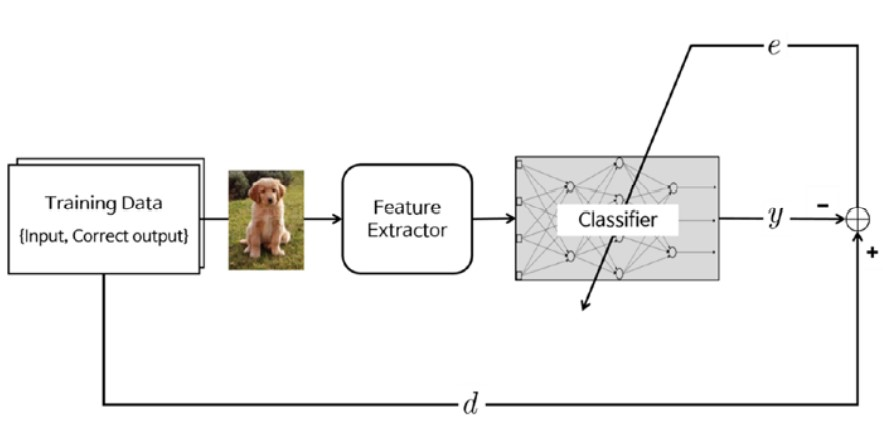
\includegraphics[scale=0.8]{gambar/imgrecog_beforconv.jpg}
    \caption{Sistem \emph{Feature Extractor} yang terpisah dari proses \emph{Machine Learning}}
    \label{fig:imgecog_beforeconv}  
\end{figure}

\par \emph{Convolutional Neural Network} mengikutsertakan proses pengambil fitur bersama dengan 
proses \emph{learning}-nya sendiri seperti yang ditunjukan pada Gambar~\ref{fig:imgrecog_afterconv}. Disinilah perbedaan dan kelebihan utama dari \emph{Convolutional Neural Network}
dimana CNN atau ConvNet ini secara \emph{automated} melakukan proses \emph{feature extraction} nya sendiri yang
menggunakan \emph{neural network} khusus yang \emph{weight} nya ditentukan melalui proses \emph{training} \cite{kim2018safety}.

\begin{figure}[ht]
    \centering
    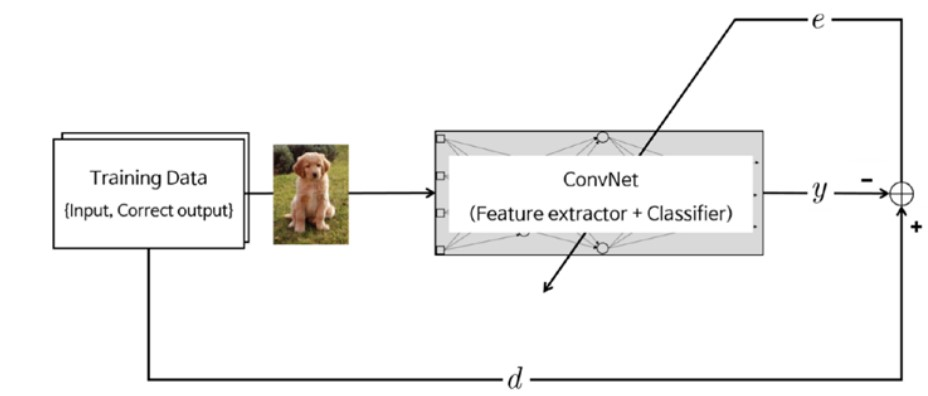
\includegraphics[scale=0.8]{gambar/imgrecog_afterconv.jpg}
    \caption{\emph{Feature Extractor} yang dilakukan bersama proses \emph{training} pada CNN}
    \label{fig:imgrecog_afterconv}  
\end{figure}



\par CNN dan MLP memiliki kemiripan dalam segi cara kerja. Perbedaan utama dari CNN dengan MLP adalah fakta
dimana CNN merepresentasikan neuron dalam bentuk 2D atau dua dimensi sedangkan pada MLP satu dimensi.
Seperti di MLP, CNN memiliki beberapa jumlah layer dengan masing - masing layer memiliki beberapa neuron.
Lalu masing - masing hubungan antar neuron di antara layer memiliki nilai bobot yang berada dalam bentuk empat dimensi
yang dimana merupakan kumpulan kernel konvolusi. Nilai bobot ini digunakan untuk melakukan operasi linear 
dari input yang dimana hasilnya ditransformasi untuk menjadi funsi aktivasi. Nama "\emph{Convolution}" pada 
CNN diambil dari operasi linearnya yang menggunakan operasi konvolusi \cite{putra2016klasifikasi}.
Pada arsitektur CNN, terdapat beberapa jenis layer yaitu \emph{Convolution Layer, Subsampling Layer, 
Fully Connected Layer}, dan \emph{Activation Layer}.

\subsection{\emph{Convolution Layer}}
\label{subsec:convolutionlayer}

\par \emph{Convolution Layer} yang merupakan layer utama dari CNN yang, sesuai namanya, melakukan proses konvolusi pada gambar 
yang lalu mengoutputkan \emph{feature map} yang dimana berguna untuk memunculkan fitur yang "unik" dari input gambar. Berbeda dengan layer pada
\emph{neural network} lainnya, \emph{convolutional layer} menggunakan \emph{convolutional filter} atau kernel untuk mengubah gambar input untuk proses konvolusi.
Kernel berkerja seperti memindai dari dari atas kiri ke kanan bawah gambar. Proses ini sebenarnya adalah aplikasi 
dari operasi konvolusi. Konvolusi merupakan pengaplikasian sebuah fungsi di suatu output secara berulang. Tujuan
diberlakukannya hal ini yaitu untuk mendapatkan fitur dari input gambar yang dimana konvolusinya akan menghasilkan
transformasi linear dari data. Bobot disini dapat diartikan sebagai spesifikasi dari kernel konvolusi yang digunakan yang
dimaksudkan untuk kernal dapat dilatih berdasarkan input yang diterima. Seperti yang diilustrasikan pada Gambar~\ref{fig:ilutrasikonvolusi} , diumpamakan sebuah
input gambar dalam bentuk matrix 5x5 berwarna hijau digunakan sebagai target konvolusi menggunakan kernel 3x3 yang diilustrasikan dengan
warna kuning dimana akan memindai dari atas kekanan bawah dengan operasi perkalian dan akan menghasilkan output hasil konvolusi yang
merupakan bentuk ektraksi fitur dari gambar input.

\begin{figure}[ht]
    \centering
    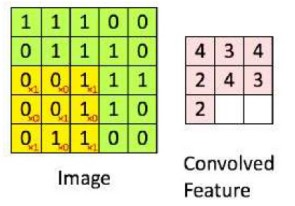
\includegraphics[scale=1]{gambar/convolution_simulation.jpg}
    \caption{Ilustrasi Konvolusi pada Matrix 5x5 dengan kernel 3x3 (Eka Putra et al., 2016)}
    \label{fig:ilutrasikonvolusi}  
\end{figure}


\subsection{\emph{Subsampling Layer}}
\label{subsec:subsamplinglayer}

\par Subsampling Layer merupakan tahap atau proses reduksi ukuran data dari suatu gambar atau citra. Tujuannya selain mengecilkan
ukurannya yaitu meningkatkan invariasi dari posisi fitur. Pada umunya metode \emph{Max Pooling} yang sering digunakan pada proses sub sampling ini daripada \emph{Mean Pooling}.
Max Pooling membagi keluaran dari convolution layer menjadi grid kecil yang dimana disini diambil \emph{max value}-nya dari dari setiap grid
tadi yang digunakan untuk menyusun gambar citra yang sudah tereduksi seperti yang ditunjukan pada Gambar~\ref{fig:prosespooling}. Menurut Springenberg et al. \cite{springenberg2014striving}, pooling layer ini digunakan
untuk mereduksi gambar sehingga lebih mudah digantikan sebuah convolution layer dengan stride yang sama dengan pooling layer
bersangkutan\cite{putra2016klasifikasi}.

\begin{figure}[ht]
    \centering
    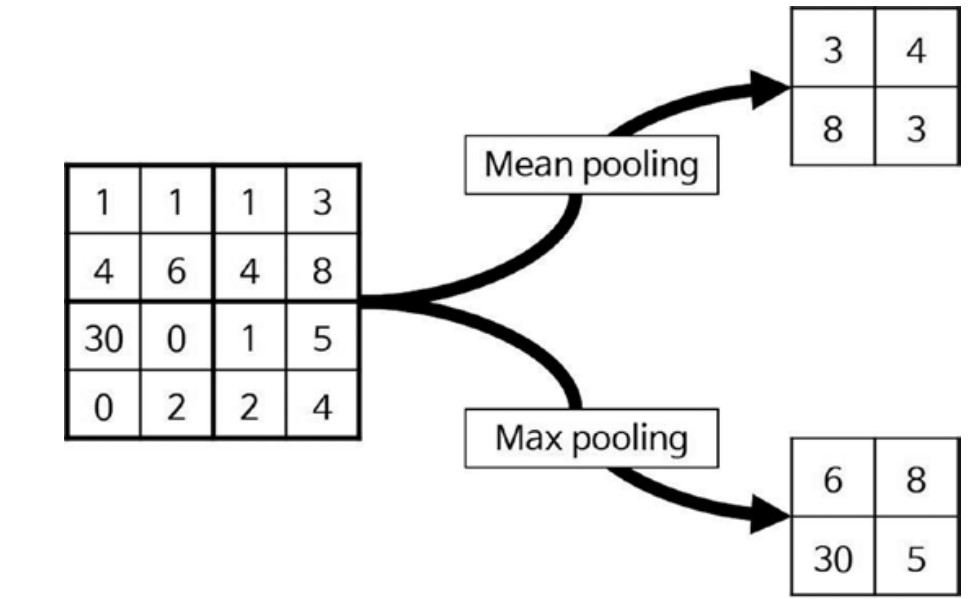
\includegraphics[scale=0.6]{gambar/pooling.jpg}
    \caption{Proses \emph{Max Pooling} dan \emph{Mean Pooling}}
    \label{fig:prosespooling}  
\end{figure}

\subsection{\emph{Fully Connected Layer}}
\label{subsec:fullyconnectedlayer}

\par \emph{Fully Connected Layer} digunakan untuk melakukan transformasi untuk dilakukan klasifikasi secara linear.
Neuron yang akan diinputkan ke FC layer ini harus ditransformasikan menjadi satu dimensi yang dimana
mengakibatkan FC layer ini hanya bisa diletakkan di akhir jaringan karena data kehilangan \emph{spatial information}-nya
sehingga menjadi \emph{irreversible} atau tidak bisa dikembalikan.

\subsection{\emph{Activation Layer}}
\label{subsec:activationlayer}

\par \emph{Activation Layer} adalah tempat dilakukannya fungsi aktivasi dimana dilakukan transformasi data input
menjadi dimensi tinggi agar memungkinakan untuk dilakukan klasifikasi\cite{putra2016klasifikasi}.


\section{Visi Komputer}
\label{sec:visikomputer}

Visi Komputer adalah bidang ilmu yang mempelajari cara untuk memproses gambar terutama dalam meniru
kemampuan manusia dalam melihat. Kemampuan seperti rekognisi wajah hingga bentuk kemampuan lain yang bahkan
melebihi kemampuan manusia. Kebanyakan riset dari bidang visi komputer di \emph{deep learning} berfokus pada
pengenalan objek atau deteksi. Bentuknya dari pengenalan atau deteksi ini bisa meliputi membuat log atau laporan
objek apa saja yang ada dalam gambar hingga memberi penandaan pada objek yang terdeteksi \cite{Goodfellow-et-al-2016}. 

\section{You Only Look Once (YOLO)}
\label{sec:youonlylookone}

\emph{You Only Look Once} atau YOLO adalah algoritma \emph{muti object detection} yang sangat cepat yang dicetuskan oleh Redmot et al pada tahun 2015
lewat buku mereka \emph{You Only Look Once: Unified, Real-Time Object Detection}\cite{redmon2016you}. Convolutional Neural Network menjadi basis dari sistem deteksi YOLO ini.
YOLO melakukan deteksi objek dengan menganggap nya sebagai pemrasalahan regresi tunggal yang diambil langsung dari \emph{pixel - pixel} yang ada
di gambar menjadi \emph{bounding box} penanda dari koordinat - koordinat dan probabilitas dari klasifikasinya. Dengan begitu
hanya perlu dilakukan satu kali pengecekan pada gambar untuk melakukan deteksi atau indentifikasi. \cite{redmon2016you}
YOLO menggabungkan beberapa komponen dari teksi objek menjadi satu neural network yang dimana menggunakan fitu-fitur
dari seluruh bagian gambar untuk memprediksi tiap \emph{bounding box} sekaligus melakukan prediksi untuk semua
\emph{bounding box} di semua tipe klasifikasi yang ada. Desain dari YOLO ini memungkinkan untuk melakukan
\emph{end to end training} dan kecepatan deteksi \emph{real time}.

\par Sistem dari YOLO sendiri membagi input gambar menjadi grid S x S. Grid disini perannya untuk 
nanti yaitu jika grid tertentu menjadi pusat dari objek maka grid tersebut yang nantinya berguna untuk deteksi objek tadi.

\par Setiap grid memprediksi tiap bound box dan nilai kemungkinan klasifikasi atau \emph{confidence score} dari \emph{bounding box} tersebut.
Nilai tersebut mewakili seberapa "yakin" model akan objek yang terdeteksi di bounding box dan seberapa akurat
prediksinya. 

\par Terdapat lima nilai prediksi yang ada pada tiap bounding box yaitu : x, y, w, h, dan \emph{confidence}.
X dan Y mewakili pusat dari bounding box. W dan H mewakili \emph{Weight} dan \emph{Height} diprediksi relatif
dari seluruh gambar. Lalu \emph{confidence score} sendiri mewakili IOU antara \emph{predicted box} dan \emph{ground truth box} \cite{redmon2016you}.

\subsection{YOLOv5}
\label{subsec:yolov5}

\begin{figure}[ht]
    \centering
    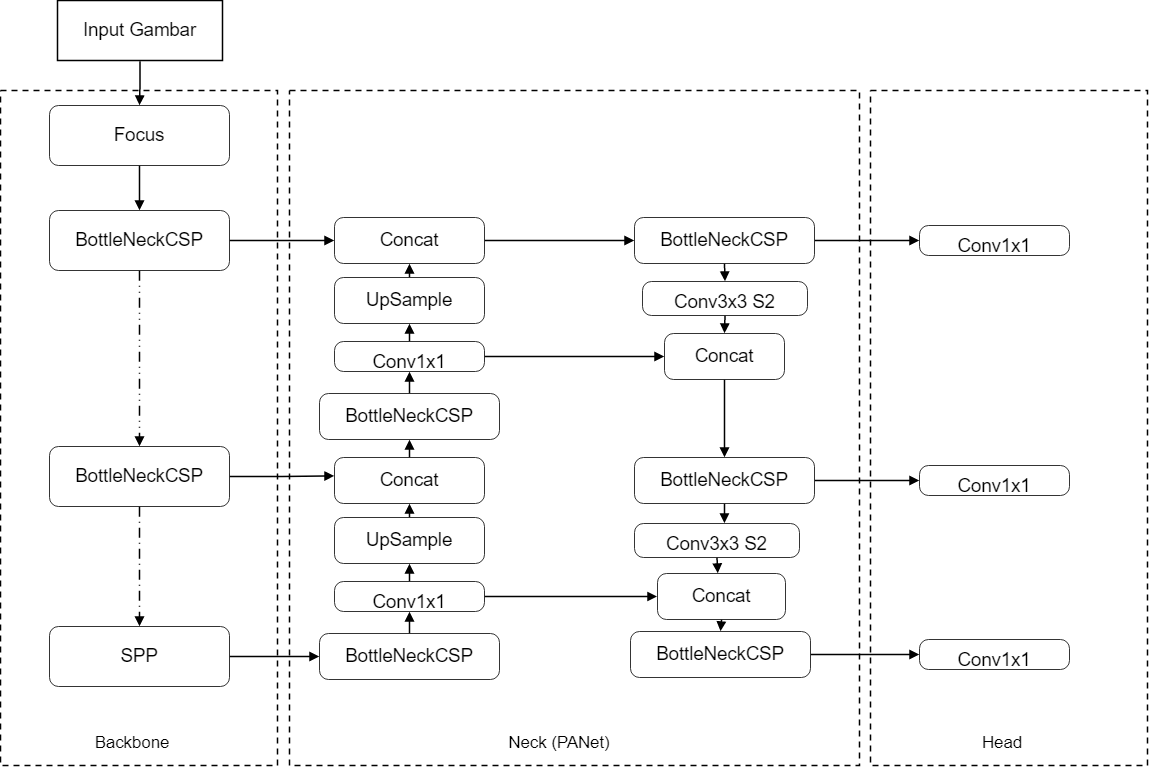
\includegraphics[scale=0.5]{gambar/yolov5 structure.png}
    \caption{Struktur Jaringan YOLOv5}
    \label{fig:yolov5network}  
\end{figure}

\par YOLOv5 merupakan versi pembaruan dari YOLO yang dicetuskan pada tahun 2020 oleh Glenn Jocher \cite{glenn_jocher_yolov5}. Berdasarkan dari \emph{repository} Github untuk YOLOv5 oleh Glenn Jocher, struktur jaringan dari YOLOv5 dibagi menjadi 3 bagian utama yaitu modul \emph{Backbone}, \emph{Neck}, dan \emph{Head}.
Seperti yang dapat dilihat di Gambar \ref{fig:yolov5network} Struktur jaringan dari YOLOv5 ini dimulai dari modul \emph{Backbone} dimana dilewati pertama oleh input gambar untuk mengekstrak fitur - fitur dari gambar yang strukturnya berbasis dari struktur \emph{Focus}, \emph{Bottleneck CSP (Cross Stage Partinal Networks)}, dan \emph{Spatial Pyramid Pooling (SPP)}.
Hasil ekstraksi fitur dari \emph{Backbone} lalu digunakan untuk menghasilkan \emph{feature pyramid} di modul \emph{Neck} yang merupakan struktur yang berbasis dari PANet (\emph{Path Aggregation Network}).
Lalu terakhir di Modul \emph{Head} dilakukan penampilan \emph{bounding box} yang meliputi beberapa informasi yaitu : kelas, koordinat, dan \emph{confidence score}.
